\documentclass[]{article}


\usepackage[utf8]{inputenc}
\usepackage{listings}
\usepackage{hyperref}
\usepackage{float}
\usepackage{graphicx}
\usepackage{subfig}
\graphicspath{ {imagenes/} }
\usepackage{xcolor}
\definecolor{RoyalBlue}{cmyk}{1, 0.50, 0, 0}
\usepackage{listings}
\lstset{language=Java,
	keywordstyle=\color{RoyalBlue},
	basicstyle=\scriptsize\ttfamily,
	commentstyle=\ttfamily\itshape\color{gray},
	stringstyle=\ttfamily,
	showstringspaces=false,
	breaklines=true,
	frameround=ffff,
	frame=single,
	rulecolor=\color{black}}



%opening
\title{Práctica 2 SS: Modelo de Simulación de Monte Carlo}
\author{José Manuel Pérez Lendínez, 26051613-l}

\begin{document}
	
	\maketitle
	
	
	\newpage
	\tableofcontents
	\newpage
	
\section{Construir un Modelo de Monte Carlo}
\subsection{Primer Modelo}

En el primer modelo tendremos que obtener la s(numero de periódicos a pedir) teniendo en cuenta que por cada periódico vendido tendremos una ganancia x y por cada periódico que no se venda una perdida y.  Para esto usaremos la siguiente función:


$$g(s, x, y, d)=\left\{\begin{array}{ll}{x * s} & { { si } d \geq s} \\ {x * d-(s-d) * y} & { { si } d<s}\end{array}\right.$$


Lo primero que haremos es ver si nos estamos aproximando al valor óptimo s. Para esto utilizaremos la distribución uniforme. Al desarrollar analíticamente el modelo con esta distribución obtenemos la siguiente formula que nos daría el valor de s optimo:

$$s^{*}=\frac{199 x-y}{2(x+y)}$$

En las siguientes tabla comparamos los valores óptimos dados por el programa y por la formula anterior.
\begin{enumerate}
	\item \textbf{ x = 10 e y = 1}
	\begin{table}[H]
		\begin{center}
			\begin{tabular}{|l|l|l|l|}
				\hline
				Nº de repeticiones & Óptimo Programa & Óptimo Formula& Mejor ganancia media\\
				\hline \hline
				$10^{4}$ & 87 & 90 &456.075
				\\ \hline
				$10^{5}$ & 92 & 90 & 449.888
				\\ \hline
				$10^{6}$ & 90 & 90 & 449.516
				\\ \hline
				$10^{7}$ & 90 & 90 & 449.587
				\\ \hline
				
			\end{tabular}
			\label{tabla:sencilla}
		\end{center}
	\end{table}

	\item \textbf{ x = 10 e y = 5}
	\begin{table}[H]
		\begin{center}
			\begin{tabular}{|l|l|l|l|}
				\hline
				Nº de repeticiones & Óptimo Programa & Óptimo Formula & Mejor ganancia media\\
				\hline \hline
				$10^{4}$ & 71 & 66 & 332.68
				\\ \hline
				$10^{5}$ & 68 & 66 & 329.106
				\\ \hline
				$10^{6}$ & 65 & 66 & 328.515
				\\ \hline
				$10^{7}$ & 66 & 66 & 328.455
				\\ \hline
				
			\end{tabular}
			\label{tabla:sencilla}
		\end{center}
	\end{table}
	\newpage
	\item \textbf{ x = 10 e y = 10}
	\begin{table}[H]
		\begin{center}
			\begin{tabular}{|l|l|l|l|}
				\hline
				Nº de repeticiones & Óptimo Programa & Óptimo Formula& Mejor ganancia media\\
				\hline \hline
				$10^{4}$ & 53 & 49 & 253.302
				\\ \hline
				$10^{5}$ & 51 & 49 & 244.638
				\\ \hline
				$10^{6}$ & 50 & 49 & 245.219
				\\ \hline
				$10^{7}$ & 49 & 49 & 244.984
				\\ \hline
				
			\end{tabular}
			\label{tabla:sencilla}
		\end{center}
	\end{table}
	
\end{enumerate}

A partir de $10^{7}$ repeticiones el resultado no suele variar en mas de 1 de diferencia con la forma analítica. En cambio en los anteriores si tenemos una mayor variación. Por tanto con un buen numero de repeticiones somos capaces de encontrar siempre un valor para s muy bueno. Con esto demostramos que nuestro modelo funciona correctamente.


Vamos ahora a probar los siguientes dos modelos de distribución para compararlos con el uniforme hecho anteriormente. Para esto vamos a realizar las mimas ejecuciones que para el modelo anterior. Como en el caso anterior vimos que los resultados eran mucho mas precisos cuando utilizamos valores altos vamos a realizar las pruebas con $10^{7}$ repeticiones siempre.

\begin{enumerate}
	\item \textbf{ x = 10 e y = 1}
	\begin{table}[H]
		\begin{center}

				\begin{tabular}{|l|l|l|}
					
					\hline
					Distribución & Óptimo programa(s) & Mejor ganancia media\\
					\hline \hline
					Uniforme &90 & 449.587
					\\ \hline
					Proporcional & 70 & 283.308
					\\ \hline
					Triangular & 79 & 468.27
					\\ \hline
					
				\end{tabular}
			
			\label{tabla:sencilla}
		\end{center}
	\end{table}
	\item \textbf{ x = 10 e y = 5}
	\begin{table}[H]
		\begin{center}
				\begin{tabular}{|l|l|l|l|l|}
					
					\hline
					 Distribución & Óptimo programa(s) & Mejor ganancia media\\
					\hline \hline
					Uniforme & 66 & 328.455
					\\ \hline
					Proporcional & 42 &  188.48
					\\ \hline
					Triangular & 59 & 386.28
					\\ \hline
					
				\end{tabular}
			
			\label{tabla:sencilla}
		\end{center}
	\end{table}
	\item \textbf{ x = 10 e y = 10}
	\begin{table}[H]
		\begin{center}
				\begin{tabular}{|l|l|l|}
					
					\hline
					Distribución & Óptimo programa(s) & Mejor ganancia media\\
					\hline \hline
					Uniforme & 49 & 244.984
					\\ \hline
					Proporcional & 29& 133.753
					\\ \hline
					Triangular & 50 & 333.4431
					\\ \hline
					
				\end{tabular}
		
			\label{tabla:sencilla}
		\end{center}
	\end{table}
\end{enumerate}

Viendo las tablas anteriores se ve claramente como siempre se da mas ganancia en la distribución triangular, seguida de la uniforme y por ultimo la proporcional.
Vamos a analizar el porque de este orden.

La triangular le da una probabilidad mayor a los valores céntricos de la distribución, disminuyendo esta probabilidad en los extremos. Esto hace que siempre consigamos una valor mas centrado asegurándonos un numero de ventas que en la mayoría de casos estará lejos de los extremos. Esto hace que pocas veces se consiga un valor para las ventas grande o pequeño, asegurándonos que la mayor parte sera céntrico y que casi siempre tendremos un buen numero de ventas. 

\begin{figure}[H]
	\centering
	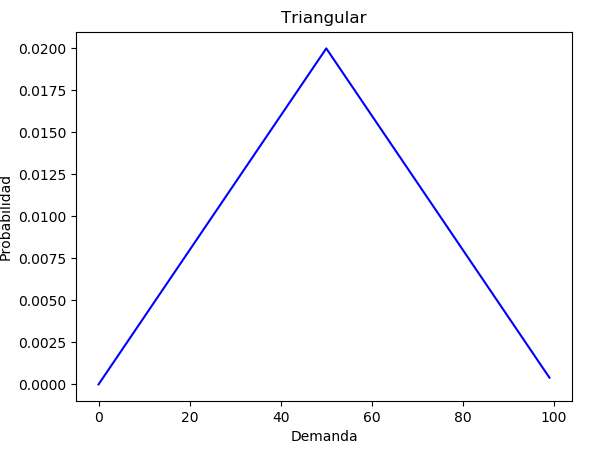
\includegraphics[width=1\linewidth]{img/screenshot002}
	\caption{}
	\label{fig:screenshot002}
\end{figure}

La proporcional nos da los peores resultados debido a que se tiene mas probabilidad a una demanda mas baja que a una demanda alta. Esto se da porque tiene una demanda decreciente desde los valores iniciales hasta los valores finales. En la grafica se ve claramente como las demandas mas altas tienen muy poca probabilidad de ser obtenida. Esto hace que siempre se vendan menos periódicos y tener unos ingresos menores, por tanto se obtendrá un valor para la demanda optimo mas cercana a valores menores que los otros dos modelos.
\begin{figure}[H]
	\centering
	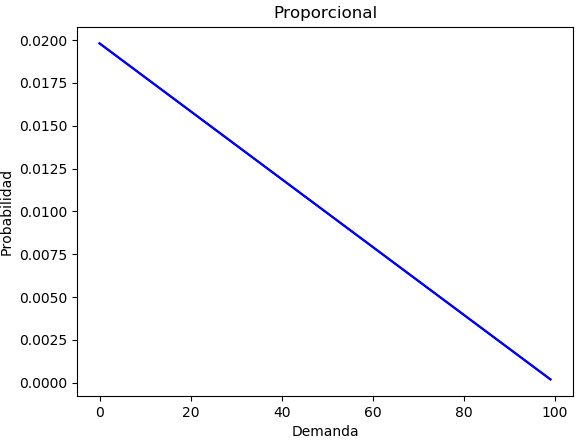
\includegraphics[width=1\linewidth]{img/screenshot001}
	\caption{}
	\label{fig:screenshot001}
\end{figure}
En estos casos como no tenemos la función que nos dice cual seria el optimo como en el caso de la uniforme, otro valor que nos puede indicar que nuestro modelos funcionan bien es que con un valor para las pérdidas (y) mayores se tiende a coger un Óptimo menor para no tener tantas pérdidas, y esto también repercute en que las ganancias bajan.
\newline

En el caso de uniforme tenemos la misma probabilidad para todas las opciones, por tanto pueden darse días que se vendan mucho y otros que se vendan menos. Esto hace mas difícil asegurarnos que cogemos un valor para s bueno en todos los casos, puesto que si se coge valores pequeños si tenemos una demanda alta en un día no podremos cubrila y en el caso de tener una demanda mas baja si tenemos un valor de s muy grande tendríamos mucha mas pérdidas. Esto hará que las  ganancias cuando tenemos unas pérdidas por unidad no vendidas pequeñas se acerque mas a los valores de la triangular puesto que podemos arriesgarnos a pedir mas unidades. En cambio cuando las pérdidas por unidad no vendida son mas alta, nos acercaremos mas a las ganancias de la proporcional al tener un coste en las pérdidas mayor.

\subsection{Primera modificación}

El fichero que contiene esta primera modificación es ModeloMontecarloM1. En esta modificación se cambia el parámetro y (perdida por unidad no vendida) por un gasto fijo por devolución(z). Este gasto fijo sera el precio que tendrá devolver cualquier numero de periódicos no vendidos. Siempre tengamos periódicos sobrantes se pagara este gasto. La función seria la siguiente:



$$
g(s, x, y, d)=\left\{\begin{array}{ll}{x * s} & { { si\ } d \geq s} \\ {x * d-z} & { { si \ } d<s}\end{array}\right.
$$

Solo es necesario cambiar la siguiente parte del condigo:
\begin{figure}[H]
	\centering
	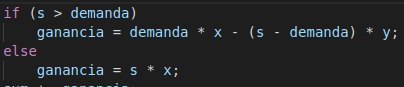
\includegraphics[width=1\linewidth]{img/screenshot003}
	\caption{}
\end{figure}

Se añade en la parte del if donde miramos si hay periódicos sobrantes la resta del precio de devolución. Quedando de la siguiente manera:

\begin{figure}[H]
	\centering
	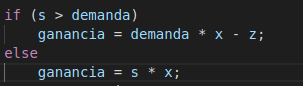
\includegraphics[width=1\linewidth]{img/screenshot005}
	\caption{}
	\label{fig:screenshot005}
\end{figure}

Vamos a analizar como cambian los ejemplos anteriores con este nuevo cambio. Se repeteria un total de $10^{7}$

\begin{enumerate}
	\item \textbf{ x = 10 e y = 1}
	\begin{table}[H]
		\begin{center}
			
			\begin{tabular}{|l|l|l|}
				
				\hline
				Distribución & Óptimo programa(s) & Mejor ganancia media\\
				\hline \hline
				Uniforme & 99 & 494.061
				\\ \hline
				Proporcional &  & 
				\\ \hline
				Triangular &  &
				\\ \hline
				
			\end{tabular}
			
			\label{tabla:sencilla}
		\end{center}
	\end{table}
	\item \textbf{ x = 10 e y = 5}
	\begin{table}[H]
		\begin{center}
			\begin{tabular}{|l|l|l|l|l|}
				
				\hline
				Distribución & Óptimo programa(s) & Mejor ganancia media\\
				\hline \hline
				Uniforme & 66 & 328.455
				\\ \hline
				Proporcional & 42 &  188.48
				\\ \hline
				Triangular & 59 & 386.28
				\\ \hline
				
			\end{tabular}
			
			\label{tabla:sencilla}
		\end{center}
	\end{table}
	\item \textbf{ x = 10 e y = 10}
	\begin{table}[H]
		\begin{center}
			\begin{tabular}{|l|l|l|}
				
				\hline
				Distribución & Óptimo programa(s) & Mejor ganancia media\\
				\hline \hline
				Uniforme & 49 & 244.984
				\\ \hline
				Proporcional & 29& 133.753
				\\ \hline
				Triangular & 50 & 333.4431
				\\ \hline
				
			\end{tabular}
			
			\label{tabla:sencilla}
		\end{center}
	\end{table}
\end{enumerate}




 
 
	
\end{document}
